\chapter{$S$-Duality and Line Defects in the Twisted 4D Theory\label{ch:finale}}

The aim of this chapter is to first develop for the reader a picture of $\mathcal N = 4$ Supersymmetric Yang-Mills (SYM) theory together with its topological twists. With this, we bring together the ideas of the previous chapters and study the actions of line defects on the categories of boundary conditions of two topological twists of $\mathcal N=4$ SYM.

\section{Setting the Stage} % (fold)
\label{sec:setting_the_stage}

\subsection{Reduction from Ten Dimensions} % (fold)
\label{sub:reduction_from_ten_dimensions}

One of the simplest ways to arrive at 4D $\mathcal N=4$ SYM is to begin with gauge theory in 10 dimensions with gauge group $G$ \cite{kapustin2006}. In the 10D theory, we have two fields, $A_{10D}$ and $\lambda$. $A_{10D}$ is a connection on a principal $G$-bundle $P$ while $\lambda$ transforms as what physicists would call a ``positive chirality spinor with values in the adjoint representation'', so $\lambda \in \Gamma(M, S^+ \otimes \ad P)$. We have $F_{10D} = \dd_{A_{10D}} A_{10D}$.

``Bosonic'' will be taken to mean terms consisting of only the connection $A_{10D}$ and its derivatives. ``Ferminionic'' will be taken to mean terms involving a the spinor $\lambda$. For more information and motivation see \cite{schwartz2014}.

The generator of supersymmetry is a spinor in $S^+$. This theory has $16$ supercharges $Q_a$. The \emph{supersymmetric variation} of the fields are given by:
\[
\begin{aligned}
	\sum_a [\epsilon^a Q_a, {A_{10D}}_I] &= i \overline \epsilon \Gamma_I \lambda\\
	\sum_a [\epsilon^a Q_a, \lambda] &= \Gamma^{IJ} {F_{10D}}_{IJ} \epsilon
\end{aligned}	
\]
The action here is:
\begin{equation}
	S = \frac{1}{e^2} \int \tr \left(F_{10D} \wedge \star F_{10D} - i \overline \lambda \Gamma \dd_A \lambda \right) 
\end{equation}

The reduction to 4 dimensions is done in a similar manner to how we proceeded in Chapter~\ref{ch:monopoles}. Namely, we assume all fields are independent of the last six direction. This gives us a connection $A =A_\mu d^\mu$ in 4D together with six scalar fields $\phi_i$. The curvature $F_{10}$ decomposes into three terms. The first is the curvature in 4D, $F$, the second consists of covariant derivatives of the $\phi_i$, $\dd_A \phi_i$, and the last consists of commutators $[\phi_i, \phi_j]$. All together, the bosonic part of the action can be written in physics convention as:
\begin{equation}
	\frac{1}{e^2} \int_M \tr\left( F \wedge \star F + \sum_i \dd_A \phi \wedge \star (\dd_A \phi) +  \sum_{i < j} [\phi_i, \phi_j]^2 \mathrm{Vol}_M \right)
\end{equation}
The fermionic part can be similarly decomposed into four spinors $\lambda^a$ transforming in $\ad(E) \otimes S^+$ and four spinors $\bar \lambda_a$ transforming in $\ad(E) \otimes S^-$. In Minkowski signature $\lambda$ and $\bar \lambda$ are conjugates but in Euclidean signature they are independent \cite{kapustin2008}.

The reduced 4D theory gains an $\mathrm{Spin}(6)$ symmetry acting on the fields which is in fact the $R$ symmetry group from Section~\ref{sec:supersymmetry}. The scalar fields $\phi_i$ transform in the vector representation of this group, while the $\lambda$ and $\bar \lambda$ transform as spinors and dual spinors of this group as well.

% \begin{equation}
% 	S = \frac{1}{e^2} \int dx^4 \tr\left( \frac{1}{2} F_{\mu \nu} F^{\mu \nu} + \sum_i D_\mu \phi^i D^\mu \phi_i + \frac12 \sum_{i,j} [\phi_i, \phi_j]^2 \right)
% \end{equation}
On $M=\rr^4$ the theory has 16 supersymmetries $\overline Q_{a, \alpha}$ and $Q^a_{\cdot \alpha}$ transforming as spinors and dual spinors in $\mathrm{Spin}(6)$ as well as for the spacetime structure group $\mathrm{Spin}(4)$.

There is also a parameter $\frac{1}{8\pi} \int_M \theta F \wedge F$ that can be added to the action where $\theta$ is called the \textbf{instanton angle}. By the usual Chern theory arguments (see Section~\ref{sub:the_instanton_number}), this depend only on the topology of the principal $G$-bundle of the gauge theory.

\begin{phys}
	$\mathcal N=4$ Super-Yang Mills theory is the field unique theory of maximal supersymmmetry in four dimensions.
\end{phys}

Further, this theory is \emph{scale invariant}. By the usual arguments \cite{schwartz2014}, it is easy to see that the mass dimension of the coupling constant $e$ must be 0. Scale invariance, together with the poincare symmetry of $\rr^4$ combine in this case to form a \emph{conformally invariant} theory known as a \textbf{conformal field theory}. For an exposition on conformal field theory in dimensions greater than two, see \cite{simmons2016}. This conformal invariance will be \emph{crucial} for the necessary duality to make sense, as otherwise the nontrivial renormalization flow would violate the Montonen-Olive duality between electric and magnetic charge, discussed below and summarized in depth in \cite{kapustin2008}.


% subsection reduction_from_ten_dimensions (end)

\subsection{Montonen-Olive Duality} % (fold)
\label{sub:montonen_olive_duality}

	\begin{concept}[Montonen-Olive Duality]
		In 4D $\mathcal N = 4$ supersymmetric Yang-Mills theory with gauge group $G$ and complex coupling constant $\tau$, any correlator of observables
		\[
			\left< \mathcal O_1 \dots \mathcal O_n \right>_{\tau, G} := \int \mathcal{D}\{ Fields \}\, \mathcal O_1 \dots \mathcal O_n \, e^{-S}
		\]
		can be rewritten in terms of Yang-Mills theory with inverse coupling constant $-1/\tau$ on the Langlands dual group $\check G$ as a correlator of dual operators $\tilde {\mathcal O_1} \dots \tilde {\mathcal O_n}$
		\[
			\left< \mathcal O_1 \dots \mathcal O_n \right>_{\tau, G} = \left< \tilde{\mathcal O_1} \dots \mathcal O_n \right>_{-1/\tau, \check G}.
		\]
	\end{concept}
	
% subsection montonen_olive_duality (end)

\subsection{Topological Twisting} % (fold)
\label{sub:topological_twisting}

	First recall from Chapter \ref{ch:phys} Section \ref{sec:supersymmetry} the following definition: 
	\begin{defn}[Subsector]
		Given a supersymmetry operator $Q$ such that $Q^2 = \frac{1}{2} [Q, Q] = 0$, we define the subsector of our theory $\mathcal E$ by the set of $Q$ invariants, and denote this as $(\mathcal E, [Q, -])$.
		
		Slightly more precisely, $[Q, -]$ defines a differential operator, and the ``observables'' become exactly those gauge-invariant quantities annihilated by $Q$ modulo those that are $Q$-exact.
	\end{defn}

	\begin{phys}[Topological Twist]
		Given a supersymmetric (SUSY) field theory $\mathcal E$, a topological twist is a procedure for extracting a sector of $\mathcal E$ that depends only on the topology of the spacetime manifold. The resulting field theory is \textbf{topological} in the definition of Section~\ref{sec:topological_quantum_field_theory}
	\end{phys}
	In general this involves a homomorphism from the universal cover of the structure group of the spacetime tangent space $TM$ to the R-symmetry group. For our four-dimensional $\mathcal N = 4$ case this is
	$$\rho : \mathrm{Spin}(4) \to \mathrm{Spin}(6)$$
	This redefines how the fields transform under the cover of the Lorentz group, $\mathrm{Spin}(4)$. 
	
	The twist that will give us the geometric Langlands duality comes from considering first the following equivalence-class of obvious embeddings.
	$$\mathrm{Spin}(4)/\zz_2 = \SO(4) \hookrightarrow \SO(6) = \mathrm{Spin}(6)/\zz_2$$
	given by:
	\[
		\begin{pmatrix}
			* & * & * & * & 0 & 0 \\
			* & * & * & * & 0 & 0 \\
			* & * & * & * & 0 & 0 \\
			* & * & * & * & 0 & 0 \\
			0 & 0 & 0 & 0 & 1 & 0 \\
			0 & 0 & 0 & 0 & 0 & 1
		\end{pmatrix}.
	\]
	This embedding will then have a $\zz_2$ lift giving our desired $\rho$. 
	
	Another way to get this embedding is to note that by the accidental isomorphisms, $\mathrm{Spin}(6) \cong \SU(4)$ and $\mathrm{Spin}(4) \cong \SU(2)_L \times \SU(2)_R$, which embeds block-diagonally into $\SU(4)$ as
	\[
		\begin{pmatrix}
			\SU(2)_L & 0 \\
			0 & \SU(2)_R
		\end{pmatrix}.
	\]
	
	After twisting by $\rho$, the group $\mathrm{Spin}(4)$ acts differently on the supersymmetry generators. In particular, of the 16 generators, one of the left-handed and one of the right-handed supersymmetries become scalars under the new action of $\mathrm{Spin}(4)$. We thus get scalars $Q_l, Q_r$, and any (complex) linear combination of these gives rise to a different ``sector'' of invariants\footnote{For a more detailed overview of what is meant by this language, the reader is invited to consult a textbook on quantum field theory discussing the BRST quantization scheme. \cite{van2005aspects} and \cite{weinberg1995quantum} are good resources for this}. Clearly overall scaling does not matter in defining the invariant fields, so we have $\mathbb P^1 (\mathbb C)$ of subsectors to chose from.
	
	Upon a choice of $Q = u Q_l + v Q_r$, after some manipulation, one can rewrite the Yang-Mills action as:
	\begin{equation}
		S = \{ Q , V \} + \frac{i \theta}{8\pi^2} \int_M \tr(F \wedge F) + \frac{i}{4\pi} \frac{v^2-u^2}{v^2+u^2} \int_M \tr (F \wedge F).
	\end{equation}
	Here $V$ is some relatively complicated gauge invariant function of the fields that will not matter in the observables in the BRST-quantized theory, since it contributes a $Q$-exact term. Note that though there is metric dependence in $V$, the remaining terms involve only $\int_M \tr (F \wedge F)$, which we know to be metric independent, depending only on the topology of the principal bundle. 
	
	\begin{fact}
		Any such sector obtained by a choice of $Q$ defines a theory that is independent of the Riemannian metric (i.e. diffeomorphism invariant). Further, this topological theory can be defined on a general curved four-manifold $M$.
	\end{fact}
	
	In general, we can bundle $\frac{\theta}{2\pi} +  \frac{v^2-u^2}{v^2+u^2}$ into a single parameter $\Psi$ known as the ``canonical parameter'' by Kapustin and Witten \cite{kapustin2006} and write:
	\[
		S = \{ Q, V\} + \frac{i \Psi}{4\pi} \int_M \tr (F \wedge F).
	\]
	We see that $\mathcal N = 4$ super Yang-Mills theory has a $\mathbb{CP}^1$ family of topological twists. 
	Two of these will be relevant here, known as the $\hat A$-model and the $\hat B$-model\footnote{This notation comes from the fact that, upon compactification down to two dimensions, these models become the $A$ and $B$ topological sigma models discussed before}. % This twisting introduces an asymmetry between $G$ and $\check G$.
	
% subsection topological_twisting (end)

\subsection{Equations of Motion in the Topologically Twisted Theory} % (fold)
\label{sub:equations_of_motion_in_the_topologically_twisted_theory}

	It is worth understanding how the field in the topologically twisted theory transform, and what constraint this puts on their configuration space and equations of motion. 

	Firstly, $A$ had trivial action under the $\Spin(6)$ subgroup, so the twist will not change how it transforms. The six scalar fields will combine into two distinct fields. One of them is a 1-form valued in $\ad P$, which will be denoted $\phi$ and the other two combine to form a complex scalar field $\sigma$ valued in the complexification of the adjoint bundle. The fermions combine into a 2-form, two 1-forms, and two scalars, but this will not be as important in the story we aim to explain. 
	
	For $Q = u Q_l + v Q_r$, define $t = v/u$. The equations of motion generically give
	\begin{equation}
		\begin{aligned}
			(F - \phi \wedge \phi + t D_\phi)^+ &= 0\\
			(F - \phi \wedge \phi - t^{-1} D_\phi)^- &= 0\\
			D \star \phi &= 0\\
			\sigma = 0
		\end{aligned}
	\end{equation}
	where $(\cdot)^+$ and $(\cdot)^-$ as in Chapter~\ref{ch:instantons} denote the self-dual and anti-self-dual parts of a given 2-form. 
	
	Our situations of interest are at $t=1$ and $t=i$. Note that at $t = i$, $\Psi = \infty$ and the $\theta$ parameter does not enter into the QFT. On the other hand, for $t = 1$, we get $\Psi = \theta/2\pi$. Thus, we can map a theory with $t=1, \theta=0$ to a theory with $t = i, \theta = 0$ by $\Psi \to -1/\Psi$ and also replacing $G$ with $\check G$.
	
	For $t = 1$ we get
	\[
	\begin{aligned}
		(F - \phi \wedge \phi + D_\phi)^+ &= 0\\
		(F - \phi \wedge \phi - D_\phi)^- &= 0\\
		D \star \phi &= 0.
	\end{aligned}	
	\]
	The first  two equations imply that
	\[
	\begin{aligned}
		\star F - \star \phi \wedge \phi + \star D_\phi &= - F + \phi \wedge \phi - D_\phi\\
		\star F - \star \phi \wedge \phi - \star D_\phi &= F - \phi \wedge \phi - D_\phi\\
	\end{aligned}		
	\]
	which in turn implies that our equations of motion can just be written as:
	\begin{equation}
		F - \phi \wedge \phi + \star D \phi = 0, \qquad D \star \phi = 0.
	\end{equation}
	It is from these equations that, after appropriate restriction to a 3-manifold, we will obtain the Bogomolny equations for monopoles.
	
	
	On the other hand, at $t=i$ we get
	\[
	\begin{aligned}
		F - \phi \wedge \phi + i D_\phi &= 0\\
		D \star \phi &= 0
	\end{aligned}	
	\]
	Upon redefining the connection to a complex connection $\mathcal A := A + i \phi$ we see that this first condition is a flatness condition on a new curvature tensor $\mathcal F := \dd_{\mathcal A} \mathcal A$.  If we allow for the complexified gauge group $\mathcal G_\cc$ to act on this field theory, the equation $D \star \phi = 0$ can be ignored and the space of solutions can be equivalently identified with the solutions to $\mathcal F = 0$ modulo \emph{complex gauge}. Following the notation of \cite{kapustin2008}, this space of field configurations will be called $\mathcal M_{flat}(G, M)$. It is here that the connection to the Langlands program is most immediate.
	
	A flat connection on a vector bundle $E \to M$ is the same as a \emph{local system} in algebraic geometry, which in turn is equivalent to a representation of the fundamental group $\pi_1(M) \to G$.
	 This space will thus capture the geometric object $\mathrm{Flat}_{\check G}$ on the Galois side. Here $M$ is a four-manifold, while in the Langlands correspondence our object of study was a . The solution is to take $M = C \times \Sigma$ for a closed complex curve $C$ and 2-manifold $\Sigma$ (generally with boundary) and perform a dimensional reduction from this topologically twisted theory to a nonlinear sigma model on $\Sigma$ valued in $\mathcal M_{flat}(G, C)$.
	 Our aim is to explore the role of Wilson lines on this space, so for a more in-depth exposition see the standard references \cite{kapustin2006, kapustin2008}. We will revisit this idea, however, in later sections. 
	
	 % The Montonen-olive duality will exchange $t=1$ with $t=i$. For the $t=1$ theory, the moduli space of solutions for these equations is called the \textbf{Hitchin moduli space} and denoted by $\mathcal M_{H}(G, M)$.

% subsection equations_of_motion_in_the_topologically_twisted_theory (end)

% section setting_the_stage (end)


\section{Wilson Lines} % (fold)
\label{sec:wilson_lines}

	\textbf{WANT TO MOTIVATE OPERATOR PRODUCT EXPANSION BETTER}

	In general, the connection 1-form, $A$, gives a way to transport data along any given vector bundle $E$ associated to a representation $R$ of $G$. This allows us to compare the values of fields operators at different points by integrating along $E$ using our connection. Recalling the definition of holonomy from Section~\ref{sub:holonomy} The result is: 
	\begin{equation}
		W_R (\gamma) = \mathrm{Tr}\, R( \mathrm{Hol}(A, \gamma))
	\end{equation}
	This classical operator is called a \textbf{Wilson line}.
	Wilson lines transform (under a general transformation $g \in \mathcal G$), as:
	\begin{equation}
		W_R(\gamma) = g(\gamma(1)) W_R(\gamma)  g(\gamma(0))^{-1}
	\end{equation}
	in the special case of $\gamma$ closed, we see this is gauge-invariant. In this case, it called a \textbf{Wilson loop}. It can be viewed as yielding an element of the group $G$ in the representation $R$. In this case, the trace of this element gives an invariant scalar quantity (known in physics as a $c$-number), and so for $\gamma$ closed we further add a trace.
	\begin{defn}[Wilson Loop]
		Given a field theory with gauge group $G$ and a finite-dimensional representation $R$ of $G$ together with a closed loop $\gamma$, we define the Wilson loop operator:
		\begin{equation}
			\mathcal W_{R}(\gamma) := \tr R( \mathrm{Hol}(A, \gamma)).
		\end{equation}
	\end{defn}
\noindent

	It is worth making a note that in general, BRST quantization on the topologically twisted theory will prohibit the existence of Wilson loops as valid operators of study. It is only in the special case of $t = \pm i$ that the modified connection $\mathcal A = A \pm i \phi$ will become a BRST invariant. 
	
	In our picture, let $M$ be a 4-manifold and let $L \subset M$ be an oriented 1-manifold embedded in $M$. On the $\hat B$-twist, we can consider taking the holonomy of the new connection $\mathcal A$ along $L$, when $L$ is closed, giving us a Wilson loop. 
	
	% \begin{prop}
% 		The $\hat B$ model condition on the flatness of $\mathcal A$ implies that the holonomy of the Wilson loop only depends on the homotopy class of $L$
% 	\end{prop} 
	
	Moreover, If $M$ has boundaries, we can let $L$ be an open 1-manifold connecting two ends of $M$. Then, the Wilson operator will give us matrix elements between the initial and final states of the theory. Because Wilson operators geometrize $\mathrm{Rep}(\check G)$, the space of physical states living on the boundary of $M$ is exactly $\check R$ for some $\check R \in \mathrm{Rep}(\check G)$. A Wilson loop connecting boundary components gives us a matrix element between initial and final vectors in $\check R$.
	
	In this topological field theory, the algebra of Wilson lines is particularly simple \cite{kapustin2006}. For $\gamma \to \gamma'$ the operator product expansion gives us that
		\begin{equation}
			\lim_{\gamma \to \gamma'} W_R (\gamma) W_{R'} (\gamma') = \sum_\alpha n_\alpha W_{R_\alpha}(L').
		\end{equation}
	From the above discussion, we should ask 
	\begin{ques}
		What is the dual operator to a Wilson line?
	\end{ques}
	From the physics viewpoint, `t Hooft showed in the 1980s that MO duality will exchange a Wilson line (a type of ``order operator'') on one side with something known as a `t Hooft line (a type of ``disorder operator'') on the other side. This physical idea arises in a broad range of contexts, and is not at all limited just to gauge theory on $\rr^4$. It is seen in statistical physics, many body theory, and even quantum spin chains \cite{kardar2007}.
	
	We can intuitively understand the insertions of `t Hooft lines in the path integral as imposing divergence conditions on the curvature form $F$ so that in local coordinates $x^1 \dots x^3$ perpendicular to the line we have
		\begin{equation}\label{eq:Amod}
			F(\vec{x}) \sim \star_3 d\left( \frac{\mu}{2r} \right)
		\end{equation}
		where $\mu$ is an element of the lie algebra $\frak g$. It turns out that for us to be able to find a gauge field $A$ whose curvature $F$ satisfies this condition, we must have that $\mu$ is a Lie algebra homomorphism $\mathbb R \to \frak g$ obtained by applying the Lie algebra functor $\mathrm{Lie}$ on a Lie group homomorphism $U(1) \to G$ to give a homomorphism $\mu: \frak u(1) \to \gg$.
		
		Another way to say this is (after using gauge freedom to conjugate $\mu$ to a particular Cartan subalgebra) that $\mu$ must lie in the coweight lattice $\Lambda_{cw}$. Note though, that if we perform a gauge transformation by
		\[
			\exp(i \pi (E_\alpha + E_{-\alpha})/\sqrt{2 \alpha^2})	
		\]
		this will send
		\[
			\mu \to \mu - 2 \alpha \alpha \cdot \mu/\left<\alpha, \alpha\right>
		\]
		which corresponds to a Weyl group action on $\mu$. This turn out to be the only degeneracy, so we have that `t Hooft operators are classified by the space:
		\[
			\Lambda_{cw}(G)/\mathcal W.
		\]
		This is also the same as 
		\[
			\Lambda_{w}(\check G)/\mathcal W.	
		\]
		Here, we can recognize this as indexing the representations of the Langlands dual group. 
		\begin{prop}
			The class of a given `t Hooft operator in the theory with gauge group $G$ are classified by the irreducible representations of $\check G$.
		\end{prop}
		
		The operator product expansion of Wilson lines captures the monoidal category structure of $\mathrm{Rep}(\check G)$. By duality, this category must also be capturing the OPE of `t Hooft lines. Can we say anything about the OPE of `t Hooft lines in terms of $G$, without reference to the dual theory?
		
		It turns out, that the answer is ``yes'', and this will give a physical interpretation of the Satake symmetries of the Langlands correspondence.

% section wilson_lines (end)

	\section{Operator Product Expansion of `t Hooft Lines}
	
	\subsection{Reduction to 3D}
	
	\textbf{NEED TO REVISE AFTER MEETING WITH PHIL}
	
	Because the operator product expansion is a local process, we can assume our base manifold looks like anything. It turns out to be fruitful to take $X = I \times C \times \mathbb R$. Here, $I$ is the unit interval $(0, 1)$, $C$ is a Riemann surface and $\mathbb R$ is regarded as the ``time'' direction and adopt a Hamiltonian point of view on $W = I \times C$. 
	
	The boundary conditions on $I$ matter here, and it turns out that in the $\hat A$ model we should consider \emph{Dirichlet} boundary conditions on one end and \emph{Neumann} boundary conditions on the other. In the language of gauge theory, Dirichlet boundary conditions demand the bundle to be trivial on that boundary, while Neumann boundary conditions allow for it to be arbitrary.
	
	Now `t Hooft lines look like points on the 3-manifold $W = I \times C$. We can locally take $\phi = \phi_4 dx^4$ so that on $W$, $\phi$ behaves as a scalar. This is the same logic as the analysis we had in Section \ref{sub:from_the_yang_mills_higgs_action_on_mathbb_r_3}.
	Then, on $W$, Equation~\eqref{eq:Amod} reduces exactly to the Bogomolny equations for monopoles:
	\[
		F = \star_3 D_A \phi.
	\]
	Let's write a local coordinate $z \in \cc$ parameterizing $C$ and $\sigma \in \mathbb R$ parameterizing $I$.
	We can gauge away $A_\sigma = 0$ exactly as we did in Section~\ref{sub:the_moduli_spaces_n_k_and_m_k} when studying the scattering transform for monopoles. These equations reduce to the following:
	\[
		\partial_\sigma A_{\bar z} = - i D_{\bar z} \phi.
	\]
	This condition can be interpreted as stating that the isomorphism class of the holomorphic $G$-bundle corresponding to the connection $A_{\bar z}$ is independent of $y$. This is because the right hand side corresponds to changing $A$ by a gauge transformation generated by $-i \phi$. Thus, gauge transforming $A \to A + i \phi$ gives us a holomorphic connection on the new $G$-bundle, putting it in the same holomorphic class.
	
	 The only place where this is violated is at the values $\sigma$ where the Bogomolny equations become singular. This is where we have the insertion of a monopole, corresponding to a `t Hooft modification of the bundle. 
	 
	 It is worth noting that this entire construction follows very closely the inverse scattering approach of Hitchin \cite{hitchin1982, atiyahhitchin1988}. In that case, the curve $C$ corresponded to the (non-compact) Riemann surface $\cc$ parameterizing the $x_1-x_2$ plane, and lines along the $x_3$ direction take the place of our $s$ variable along the unit interval $I$.
	
	\subsection{The Affine Grassmannian}
	
	\textbf{NOT FINISHED}
	
	The Langlands dual is defined to have the property that any highest weight representation $\hat \rho: \hat G \to U(1)$ is dual to a morphism $\rho: U(1) \to G$ which can be viewed as a \emph{clutching function} for a $G$ bundle on the Riemann sphere $\mathbb{CP}^1$. Complexifying this gives $\rho: G \to \cc^\times \cong \mathbb{CP}^1 \backslash \{p, q \}$, AKA gluing a trivial bundle over $\mathbb{CP}^1 \backslash \{p \}$ to a trivial bundle over $\mathbb{CP}^1 \backslash \{q \}$. This is exactly what we call a Hecke modification of type $\rho$. Every holomorphic $G$-bundle over $\mathbb{CP}^1$ arises in this way. We can recognize this space of Hecke modifications as the affine Grassmannian $Gr_G = G((z))/G[[z]]$.

	\subsection{The Space of Physical States}
	
	\textbf{NOT FINISHED}
	
	It turns out that for $\mathcal N = 4$ supersymmetric Yang Mills, the space of physical states is the (intersection) cohomology of the space of solutions to the Bogomolny equations with prescribed singularities labeled by $\check R_i, p_i$\footnote{In general, there are so-called ``instanton corrections'' to this space of states, but they are absent in this situation for reasons relating to supersymmetry.}. We denote this space by $\mathcal Z(\check R_1, p_1, \dots, \check R_k, p_k)$. Because the underlying field theory is topological, and because the space of $n$-tuples on $W$ is simply connected (so no monodromy can occur), we have that $\mathcal Z$ does not depend on the explicit positions of any of the $p_i$. Thus we can write $\mathcal H (\check R_1, \dots \check R_k) = H^*(\mathcal Z)$ and define this as the \emph{space of physical states} for this given set of line defect insertions.
	
	Further, $\mathcal Z(\check R_1, \dots \check R_k)$ turns out to topologically be a simple product $\prod_{i=1}^k \mathcal Z(\check R_i)$ where $\mathcal Z(\check R_i)$ is the same as the compactified space $\mathcal N(\check R_i)$ of Hecke modifications of type $\check R_i$, then by using the fact that \emph{the product of cohomologies is the cohomology of the product} we obtain:
	\begin{equation}
		\mathcal H(\check R_1, \dots \check R_k) = \bigotimes_{i=1}^k \mathcal H(\check R_i)
	\end{equation}
	
	This suggests that there is an isomorphism of $\check R_i$ and $\mathcal H(\check R_i)$ as vector spaces. Indeed, it can be shown that such an isomorphism is the only way for these categories of (finite dimensional) vector spaces to have the same monoidal structure.
	
	\section{The Action of Wilson Loops on Boundary Conditions}
	
	\textbf{NOT FINISHED}
	
	If we assume that $M = \Sigma \times C$ for $C$ a compact Riemann surface and $\Sigma$ a (not necessarily compact) surface with boundary, we can study loop insertions more naturally. The following is a simplified picture of the general case:

	\begin{defn}[Hitchin's Moduli Space]
		$\mathcal M_H (G, C)$ is the space of solutions to the Hitchin equations on a curve $C$. 
	\end{defn}
	If we consider $C$ to be ``small'' relative to $\Sigma$, for each point in $\Sigma$, the additional data for the field configurations on the space $C$ must give us a point in this moduli space. That is, we get a nonlinear sigma model on $\Sigma \to \mathcal M (G, C)$.
	
	Let the curve defining a (Wilson or `t Hooft) operator be $\gamma = \gamma_0 \times p$ in $\Sigma \times C$ with $p$ a point on $C$ and $\gamma_0$ a curve on $\Sigma$. Let $\partial \Sigma_0$ be a connected component of $\partial \Sigma$. A boundary condition for the field theory on $\Sigma_0$ is called a \textbf{brane}.
	
	Let $\gamma_0$ approach this boundary. On the $\hat B$ side, the insertion of a Wilson loop acts as an associative endofunctor for the category of boundary conditions on the topological sigma model on $\Sigma$ with target $\mathcal M_H (G, C)$. This target  space, with choice of complex structure $J$, can be identified with $\mathcal M_{flat} (G, C)$.
	
	\begin{figure}
		\centering
		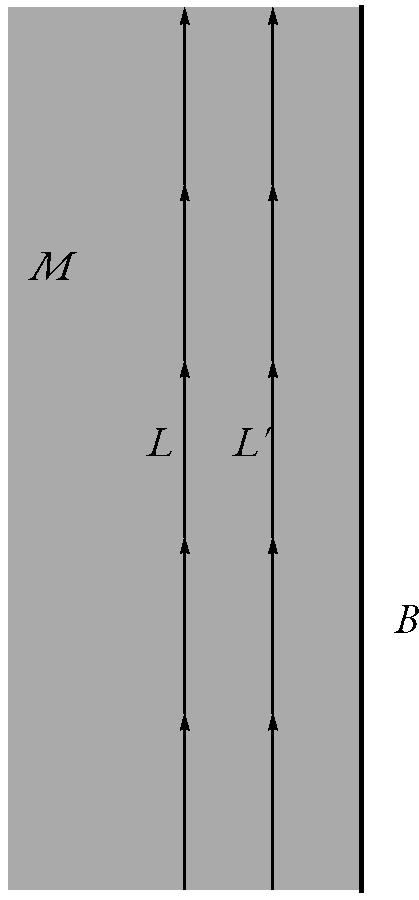
\includegraphics[scale=0.5]{figures/Wilson}
		\caption{The insertion of two Wilson lines approaching a boundary. They act associatively on the category of boundary conditions, and have actions commuting with one another.}
		\label{fig:wilson}
	\end{figure}
	
	 This functor will depend on the point $p \in C$ corresponding to the Wilson line. Consider the product $\mathcal M_{flat} (G, C) \times C$. There is a universal $G$-bundle $\mathcal E$ over this space, given by taking a point in $\mathcal M_{flat}$ and restricting the corresponding bundle to a point in $C$. 
	
	Given any coherent sheaf on $\mathcal M_{flat}$, we can tensor this with $R(\mathcal E)$. This is the action of the Wilson loop insertion on the space.
	
	Consider the structure sheaf $\mathcal O_x$ of a point $x \in \mathcal M_{flat}(\check G, C)$. For any representation $\check R$, the Wilson loop maps $\mathcal O_x$ to $\mathcal O_x \otimes \check{R}$.
	Thus $\mathcal O_x$ is an eigen-object for the functor $W_{\check R}(p)$, which acts on it by tensoring it with the vector space $\check R(\mathcal E_p)_x$. In fact, letting $p$ vary we see that it is an eigen-object for all $W_{\check R}(p)$. Another way of saying this is that the eigenvalue is the flat $\check G$-bundle $\check R(\mathcal E)_x$ on $C$.
	
	More directly, this flat bundle is obtained by taking the flat principle bundle on $C$ corresponding to $x$ and forming the associated bundle via $\check R$.
	
	The action of the `t Hooft operators is more difficult to see. They will end up acting by Hecke transformations on the space of boundary conditions. By Monotonen-Olive duality, it turns out that the brane corresponding to a fiber of the Hitchin fibration in $\mathcal M_H(G, C)$ is a common eigenobject for all operators.
	
